\documentclass{article}
\title{TDA297 Laboration 2}
\author{anordin@student.chalmers.se\quad Anders Nordin\\
        viklin@student.chalmers.se\quad Viktor Lindstr\"{o}m}
\date{\today}
\usepackage[T1]{fontenc}
\usepackage[utf8]{inputenc}
\usepackage[english]{babel}
\usepackage{verbatim}
\usepackage{enumerate}
\usepackage{steinmetz}%för att få tillgång till /phase
\usepackage{amsmath}%massa trevliga symboler
\usepackage{siunitx}%enklare notation på enheter
\usepackage{tikz}
\usetikzlibrary{arrows,decorations.pathmorphing,backgrounds,positioning,fit,petri}
\usepackage{fullpage}
\begin{document}
\maketitle
\newpage

\section{Introduction}
  This report describes some of the problems of distributed network and how to maintain total order 
  as well as causal order in a system that has reliable unicast FIFO order messaging.\\
  The report will start with a short description of the system and what algorithms used. 
  Then reliability is discussed and how the system solve integrity, validity and agreement.
  After that an explanation of how the system holds for total and causal order. Then there 
  is an explanation of how the system handle crashing processes. Lastly there is a conclusion.

\section{Description of the system}
 The system consists of N processes that communicate with each other by TCP channels.
 TCP channels gives the system reliable unicast with FIFO order. Upon this system a
 reliable total order and causal order multicast is implemented. 
 \subsection{Sequencer}
 In this system there exists a single node that is also a sequencer. All messages will 
 pass through the sequencer and the sequencer will then add a sequence number to that 
 message, and then distribute it to all nodes. The nodes will then receive the message 
 and then start flooding it to all other nodes. These events is described by Figure 
 \ref{fig1}. An important thing to note in the figure is that the sequencer is described 
 as an independent node. This is for simplification, in reality the sequencer is kept 
 within a node. \\
 \subsection{Nodes}
 The normal nodes will send its message to the sequencer, get it back with a sequence number.
 In order to then create the correct order, the messages is not delivered directly when
 it is received, but is instead put in a queue until the correct sequence number is acquired.\\
 \subsection{Example}
 Example of two functioning nodes with a sequencer. The message sent tot he sequencer is 
 represented by a wavy arrow, and the messages with a sequence number is represented by normal
 arrows.
  \begin{figure}[h]
    \centering
    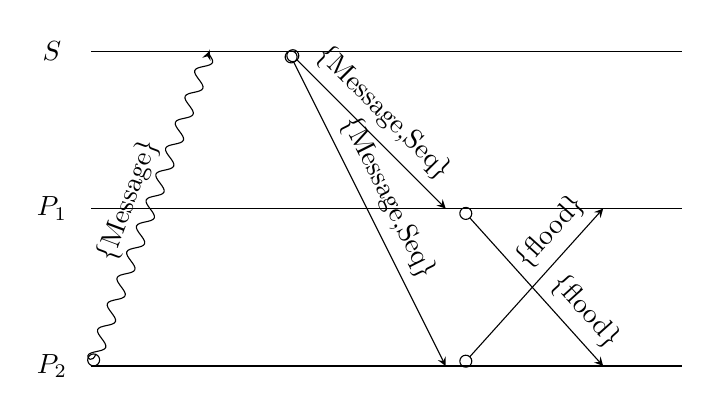
\begin{tikzpicture}
      \draw (0,0) node{$P_2$} (0.5,0) -- (8,0);
      \draw (0,2) node{$P_1$} (0.5,2) -- (8,2);
      \draw (0,4) node{$S$}   (0.5,4) -- (8,4);

      \draw [decorate, decoration=snake, o-stealth,anchor=south,sloped] (0.5,0) -- 
          node {\{Message\}}    (2,4);
      \draw (3,4)[o-stealth,anchor=south,sloped] -- 
          node {\{Message,Seq\}} (5,2);
      \draw (3,4)[o-stealth,anchor=south,sloped] -- 
          node {\{Message,Seq\}} (5,0);

      \draw (5.2,0)[o-stealth,anchor=south west,sloped] -- 
          node {\{flood\}} (7,2);
      \draw (5.2,2)[o-stealth,anchor=south west,sloped] -- 
          node {\{flood\}} (7,0);
    \end{tikzpicture}
    \caption{Example of a message being multicasted}
    \label{fig1}
  \end{figure}
  
  \subsection{Assumptions}
  The system is built upon the following assumptions:
  \label{assumption}
  \begin{itemize}
  \item Reliable unicast
  \item FIFO-order unicast
  \item No partitioning in the network
  \end{itemize}  

\section{Reliability}
  \label{reliability}
  %Short description here, proofs in subsections!
  The reliability is provided by flooding the message. By the assumptions made in \ref{assumption} we can rely on 
  that each single message sent by a working process $P_i$ to its neighbours $P_j$ to $P_n$ will be delivered.
  And hence the sequencer is the only one that sets the sequence number the number is preserved within the message.
  
\subsection{Integrity}
% What will happen when a process crash?
% We use seq nr to assure the we dont have any duplicates. Stored in set(no duplicates).
% "Each process delivers a message at most once from another process. The message must been broadcasted earlier"


\subsection{Validity}
% The set beeing delivered must contain all  msgs that have been broadcasted by correct processes"
% Flooding is the key and like we said no netwrok partions. 
% Atomic broadcast, once one peer has the msg everyone will get it by flooding principle.

\subsection{Agreement}
% All correct processes will eventually deliver same set of msgs"
% Same as validity, if it applies for one it applies for all.

\section{Ordering}
  It is important in the protocol that the order of the messages is the same 
  for all members of the network. Therefore in the following subsection it is 
  described how the protocol satisfy total and causal order.

\subsection{Total order}
  The sequencer is the only one that takes care of the ordering. 
  No one else is allowed to set a sequence numbers. If a message 
  is sent, it has to be passed to the sequencer, get a sequence 
  number, and then it is delivered back by a broadcast. When it 
  is recieved it is not delivered, it has to be put to a queue 
  untill the message with the next sequence number if found. 
  Hence there is only one node that is allowed to set sequence 
  numbers, and the  sequence numbers is unique, all the nodes 
  will get a message with a sequence number.
  
\subsection{Causal order}
\section{Fault tolerance}
  Fault tolerance in failing nodes is already described in section \ref{reliability}.
  An important notice that is not to be forgotten is the sequencer. If the sequencer 
  dies, a new sequencer has to be elected and integrity, validity and agreement will 
  still be preserved aswell as ordering.
  \subsection{Integrity}
    When a node is sending a message, one and only one, is created and then put in a queue.
    the message together with an unique id specific for that processor. When the message then is 
    received from the broadcast it is then removed. This means that if and only if a message is 
    sent, it    will be present in the sending nodes send buffer, and if and only if the message
    is broadcasted it is removed from the buffer. No where will it be duplicates.
    
  \subsection{Validity}
    If a node containing the sequencer crashes, the other nodes will place their messages in their
    send buffer and then try to send them, when they realize that the node is unreachable, a new 
    sequencer is elected. The elected node will then send a message to the other nodes updating them
    about a new sequencer is elected, and it is to this nodes the following messages should be sent.
    The nodes will then send the messages it was unable to send to the previous sequencer to the
    new sequencer, and they will then be multicasted and removed from the buffer to inform the nodes
    that the message is infact broadcasted.
  \subsection{Agreement}
    When a new sequencer is elected, the elected process will send a special message to the other nodes
    that it is the new sequencer, hence the single one is elected, and it and only itself sends the 
    messages to all other nodes to be updated, no one will be without a notion of the new leader
  \subsection{Ordering}
    If the sequencer dies, then the nodes will buffer their messages. Thiese messages 
    each process buffer while sequencer is dead will be concurrent, and no need for flooding or special
    ordering is needed. When the new sequencer is found the nodes just have to send their messages as soon
    as possible, but before anything else, to the sequencer. Hence causal order will be preserved, no one
    can recieve messages while the sequencer is dead and they will be causally concurrent. The new sequencer
    will set sequencer numbers and multicast the message exactly as before so total order is also preserved
    hence it is buffered in each node and then delivered according to sequence numbers.
    
\section{Conclusion}
\end{document}
